\chapter{Multitasking}
\label{cha:multitasking}

The goal of soft robotics is to generate a new category of robots, inspired by nature and designed to perform well on dynamic and unpredictable environments.\\
This chapter analyzes the behaviour of map-elites best performing individuals in tasks they where not designed for.
For each experiment, the fittest individuals in a certain task, which are the ones stored in the final map, have been trained in a new task.

Since the walker task observation space is different from the ones of the other two environments it is compared with, validating individuals using both the structures and the controllers already optimized and stored is impossible.
For this reason, the morphologies of the best individuals have been used with no optimization, and the controller has been re-optimized in the new environment.

Nevertheless, in the carrier and pusher tasks individuals have also been evaluated using both the body and the controller already optimized in the original task. This has been possible since the observation space of the two tasks is the same.


\section{Preliminary considerations}
Figure \ref{fig:task_comparison} displays the fitness trends of experiments in the three tasks, using MAP-Elites to optimize the design, and PPO to optimize the controller.\\
The three trends are not comparable because of the different reward definition of the three tasks.

The pusher and the carrier are expected to be good walkers, since they both have the implicit goal of learning how to walk, other than interacting with an object. The opposite is not true: even though an individual is a good walker, he might be incapable of interacting with an object, since it only learned how to walk. It might not disappoint as a pusher, as a good morphology with a strong front leg might allow it to oppose to the box resistance. The same cannot be said for carrying a box, as it requires a good conformation at the top of the robot, to prevent the box from falling.

\begin{figure}
    \centering
    \begin{subfigure}[b]{0.3\textwidth}
        \centering
        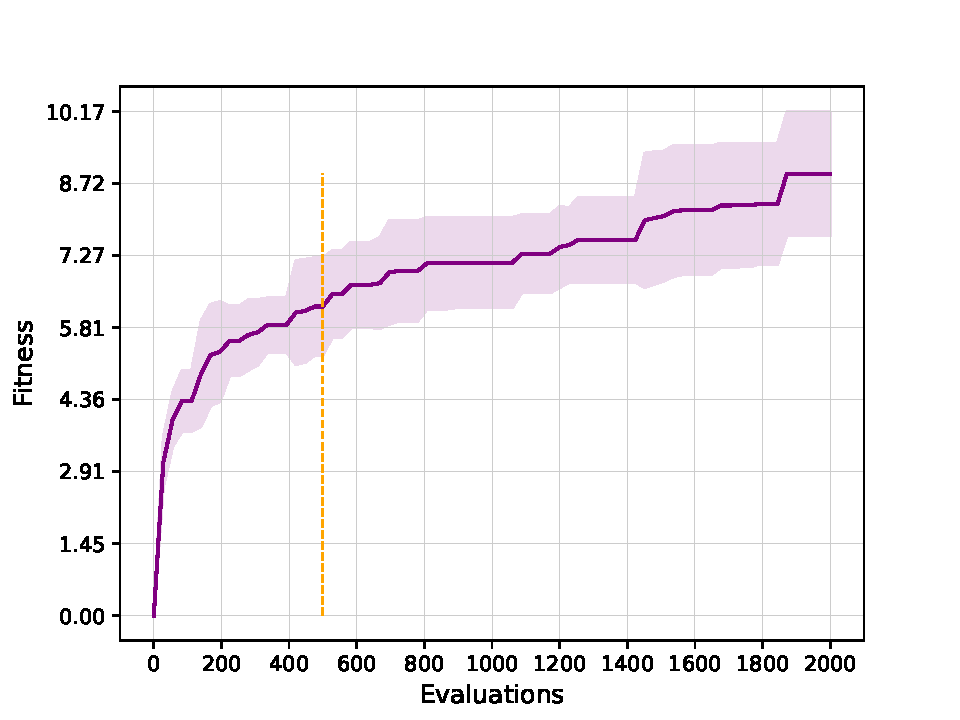
\includegraphics[scale=0.35]{images/multitasking/ft_walker.pdf}
        \caption{Walker}
    \end{subfigure}
    \begin{subfigure}[b]{0.3\textwidth}
        \centering
        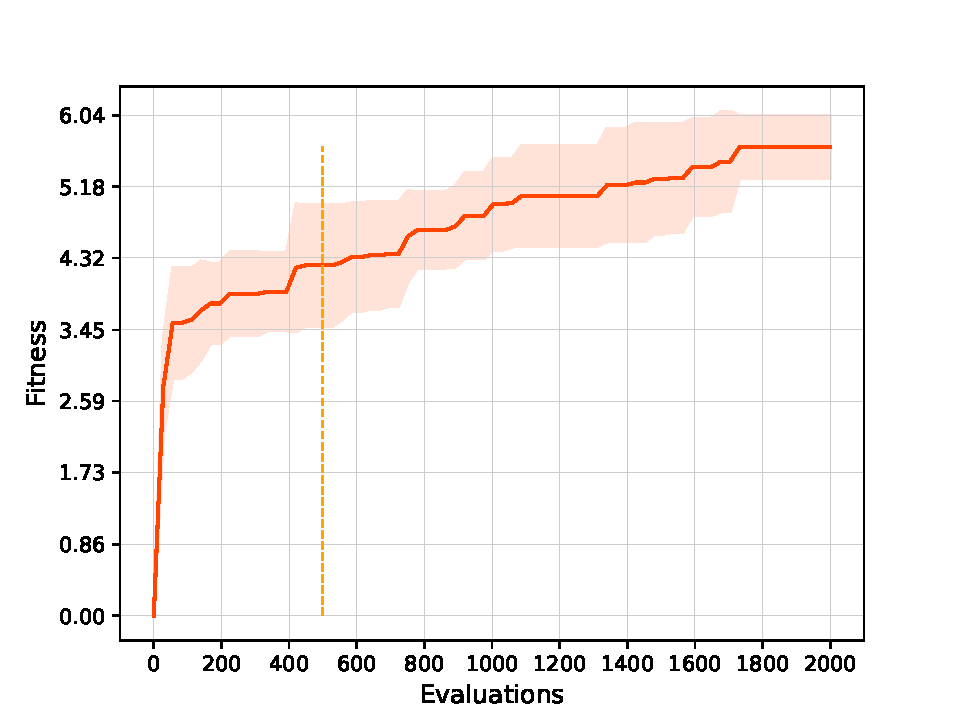
\includegraphics[scale=0.35]{images/multitasking/ft_pusher.pdf}
        \caption{Pusher}
    \end{subfigure}
    \begin{subfigure}[b]{0.3\textwidth}
        \centering
        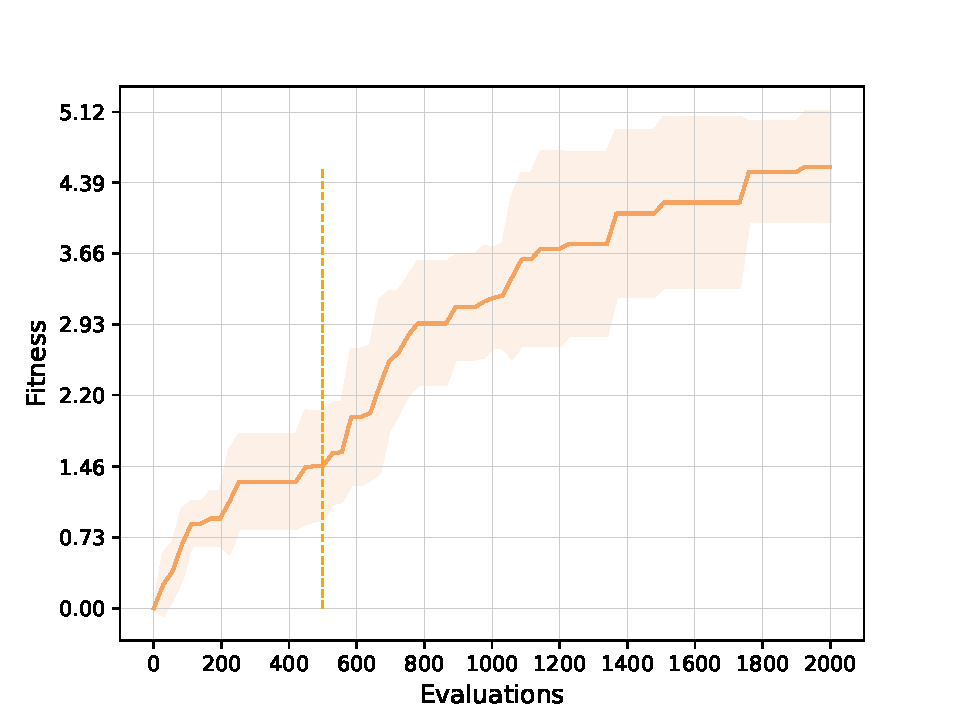
\includegraphics[scale=0.35]{images/multitasking/ft_carrier.pdf}
        \caption{Carrier}
    \end{subfigure}
    \caption{Fitness trend in the three tasks.}
    \label{fig:task_comparison}
\end{figure}


\section{Task performance comparison}
Is an individual who has only learnt how to walk able to push or carry an object? Can a pusher (carrier) carry (push) an object as far as possible? How well can pushers and carriers walk?
This section tries to answer to these questions by providing the performance map generated in a task and the ones obtained by training the same individuals in a different environment.

Note that the reward definition vary according to the task, therefore the results obtained by evaluating in different environments are not comparable.
For more details about the reward definition of the three tasks, pleas refer to Chapter \ref{cha:chapter1}.

Figure \ref{fig:walker_multitask} shows the performance maps generated by optimizing the controller of the best walker designs in the walking task itself (Map \ref{walker_a}), in the pusher and carrier task (Maps \ref{walker_b} and \ref{walker_c} respectively).\\
The obtained maps highlights that walkers might be good pushers, however the overall fitness in the carrier task is poor.\\
The results meet the expectations, since the ability of walking might help to push an object forward, but it doesn't provide any knowledge on how to carry a box.

The results of best pusher designs trained in the three tasks are shown in Figure \ref{fig:pusher_multitask}. These individuals are well able of pushing an object, for which they had been designed for, and walking forward; however, once again, they get poor results in the carrier task. The maps obtained in the first two tasks are very similar, and this is because walking is an implicit goal while learning to push a box forward.

The best carrier designs obtain interesting, but not excellent, results in the walking and pushing environment, as shown in Figure \ref{fig:carrier_multitask}. Map \ref{carrier_c} highlights that the best performing individuals in the carrier task are the ones for which the body and the controller have both been trained in that same environment.

%%%% WALKER %%%%
\begin{figure}
    \centering
    \begin{subfigure}[b]{0.3\textwidth}
         \centering
         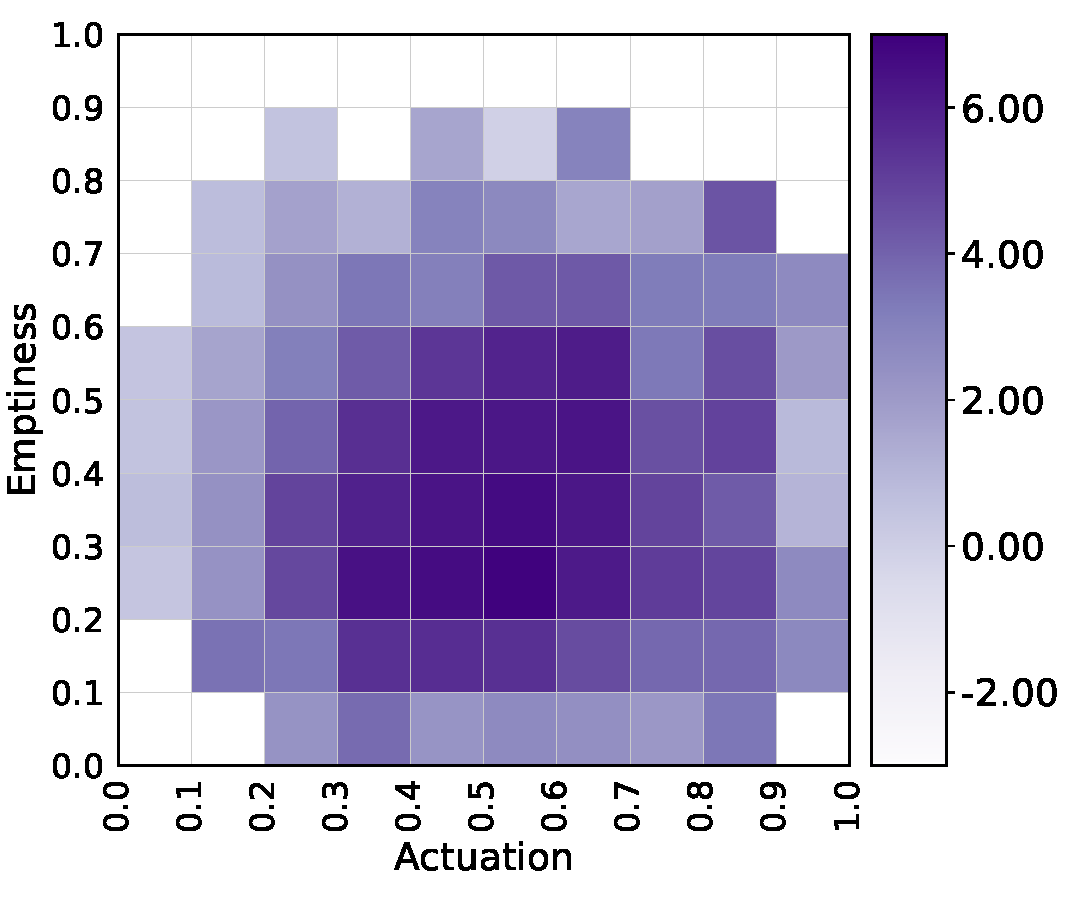
\includegraphics[scale=0.3]{images/multitasking/walker.pdf}
         \caption{Walker}
         \label{walker_a}
     \end{subfigure}
     \hfill
     \begin{subfigure}[b]{0.3\textwidth}
         \centering
         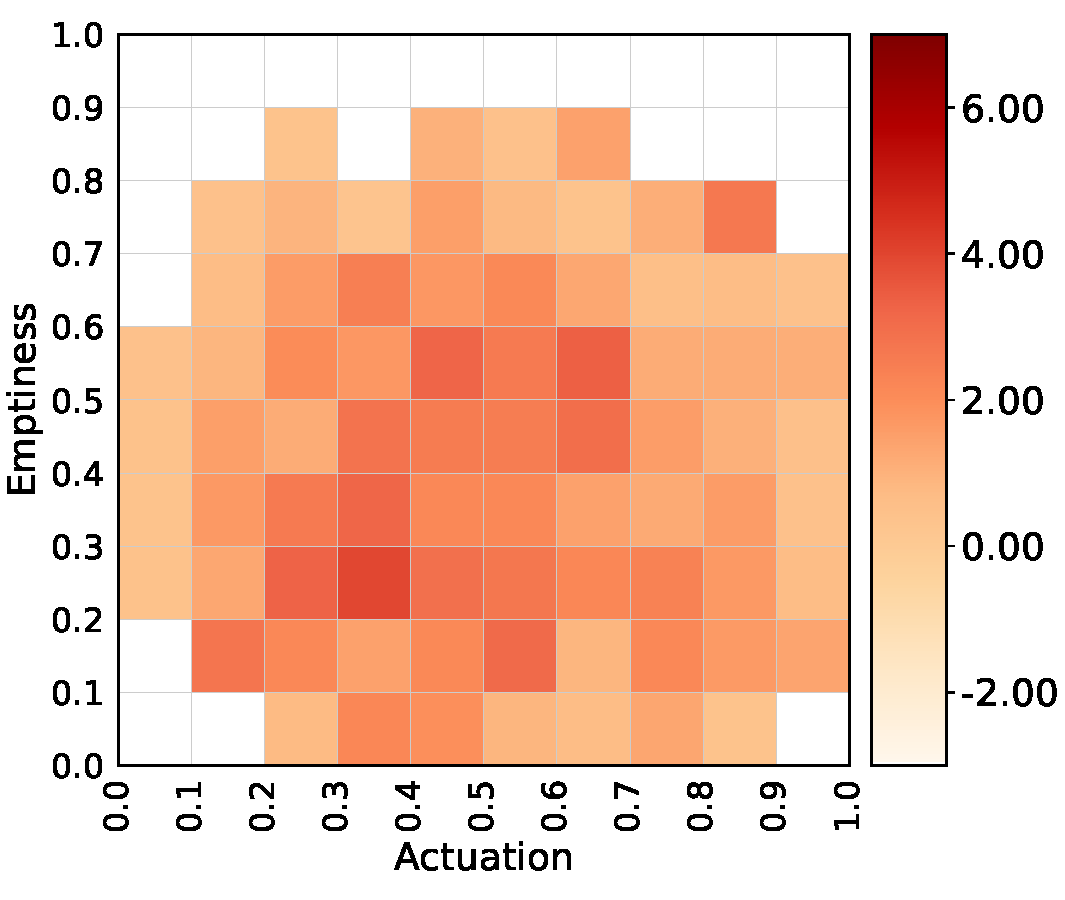
\includegraphics[scale=0.3]{images/multitasking/walker_p.pdf}
         \caption{Pusher}
         \label{walker_b}
     \end{subfigure}
     \hfill
     \begin{subfigure}[b]{0.3\textwidth}
         \centering
         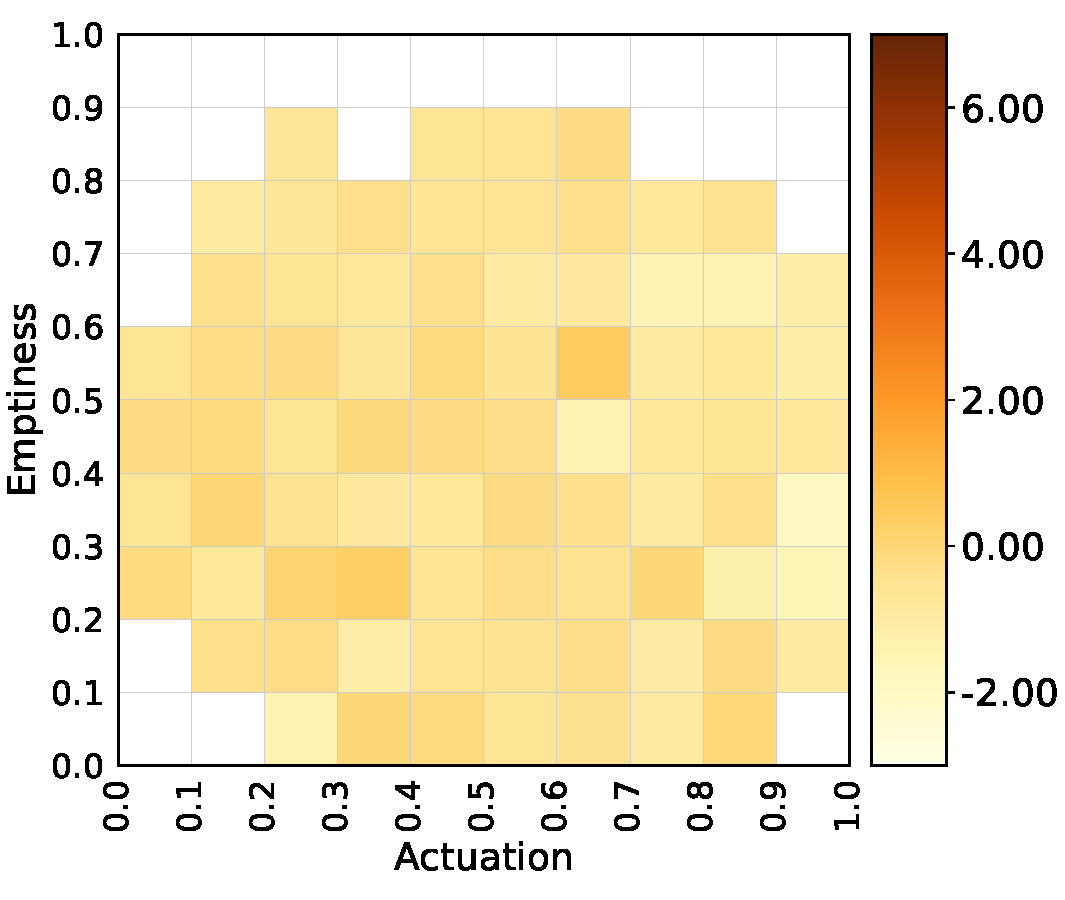
\includegraphics[scale=0.3]{images/multitasking/walker_c.pdf}
         \caption{carrier}
         \label{walker_c}
     \end{subfigure}
    \caption{Walker designs trained in the walker (a), pusher (b), carrier (c) task.
    The maps can be compared for the fitness distribution, however the obtained fitness cannot be compared, since its definition is different in the three tasks.}
    \label{fig:walker_multitask}
\end{figure}

%%%% PUSHER %%%
\begin{figure}
    \centering
    \begin{subfigure}[b]{0.3\textwidth}
         \centering
         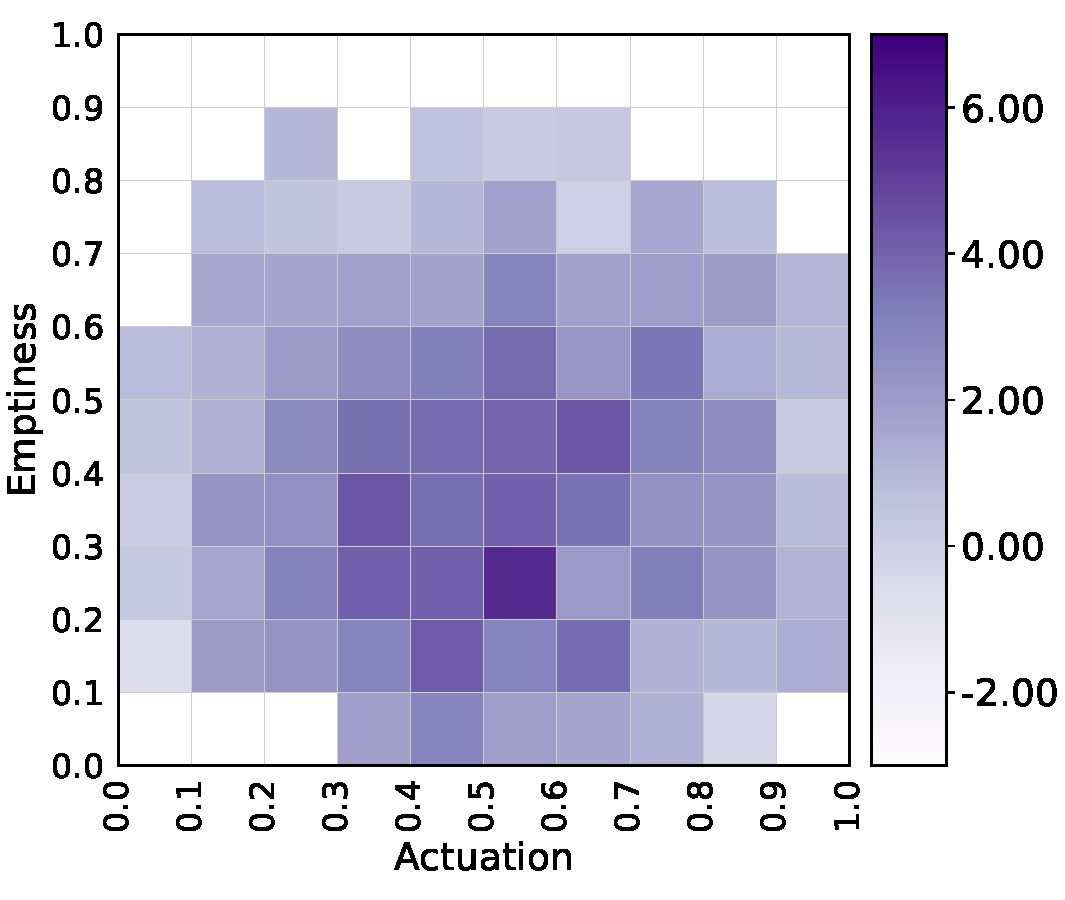
\includegraphics[scale=0.3]{images/multitasking/pusher_w.pdf}
         \caption{Walker}
         \label{pusher_a}
    \end{subfigure}
    \hfill
    \begin{subfigure}[b]{0.3\textwidth}
         \centering
         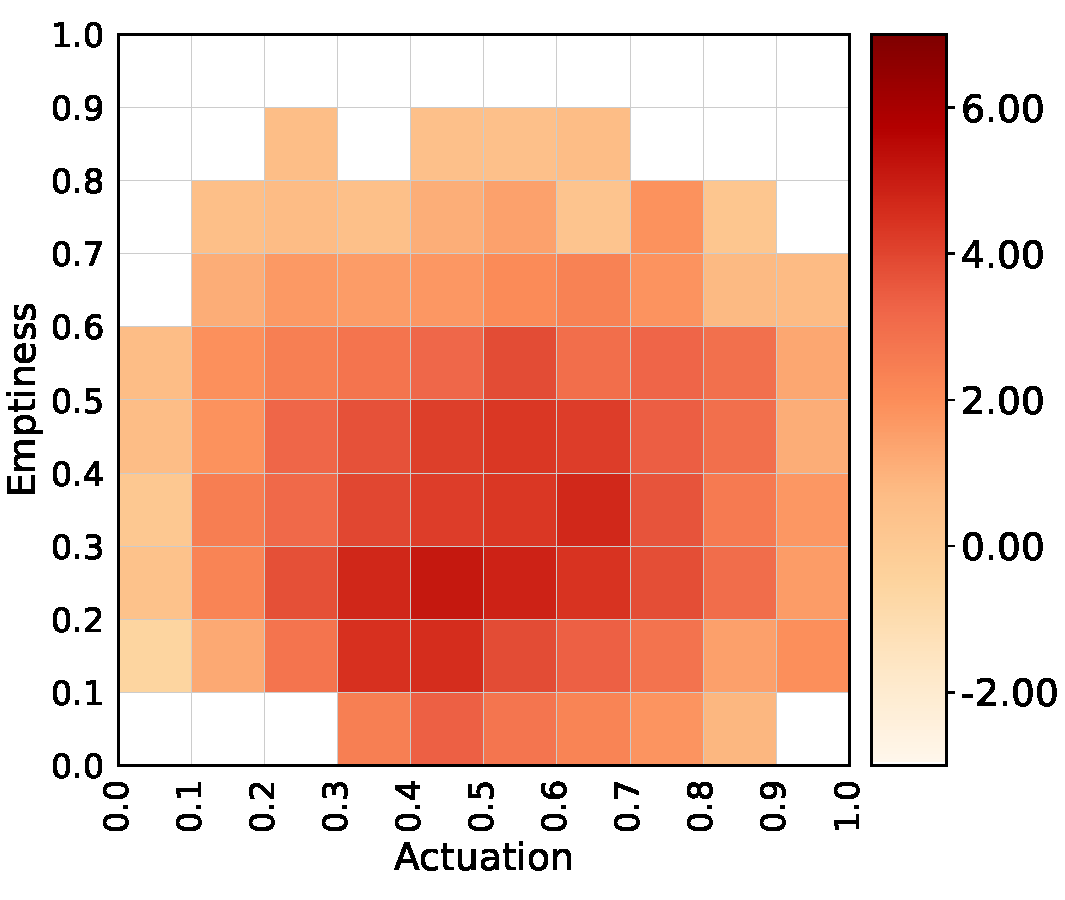
\includegraphics[scale=0.3]{images/multitasking/pusher.pdf}
         \caption{Pusher}
         \label{pusher_b}
    \end{subfigure}
    \hfill
    \begin{subfigure}[b]{0.3\textwidth}
         \centering
         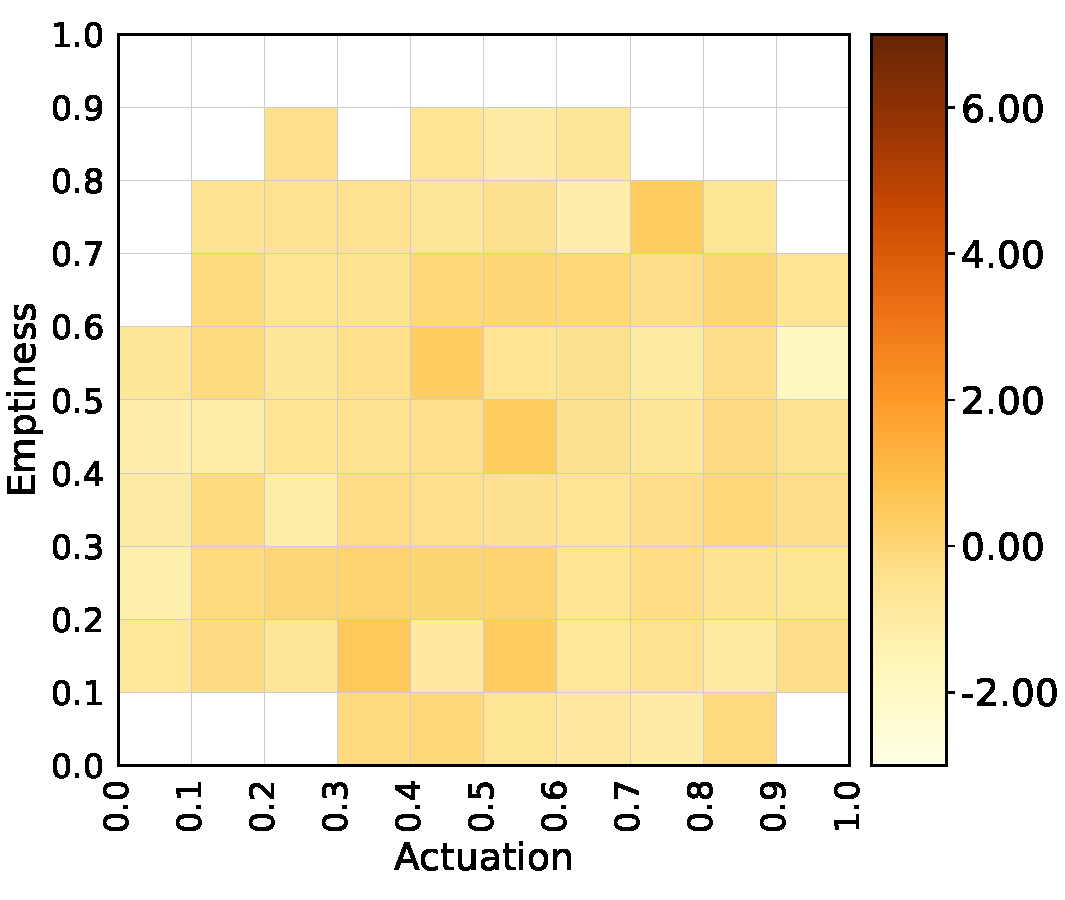
\includegraphics[scale=0.3]{images/multitasking/pusher_c.pdf}
         \caption{Carrier}
         \label{pusher_c}
    \end{subfigure}
    \caption{Pusher designs trained in the walker (a), pusher (b), carrier (c) task.
    The maps can be compared for the fitness distribution, however the obtained fitness cannot be compared, since its definition is different in the three tasks.}
    \label{fig:pusher_multitask}
\end{figure}

%%% CARRIER %%%
\begin{figure}
    \centering
    \begin{subfigure}[b]{0.3\textwidth}
         \centering
         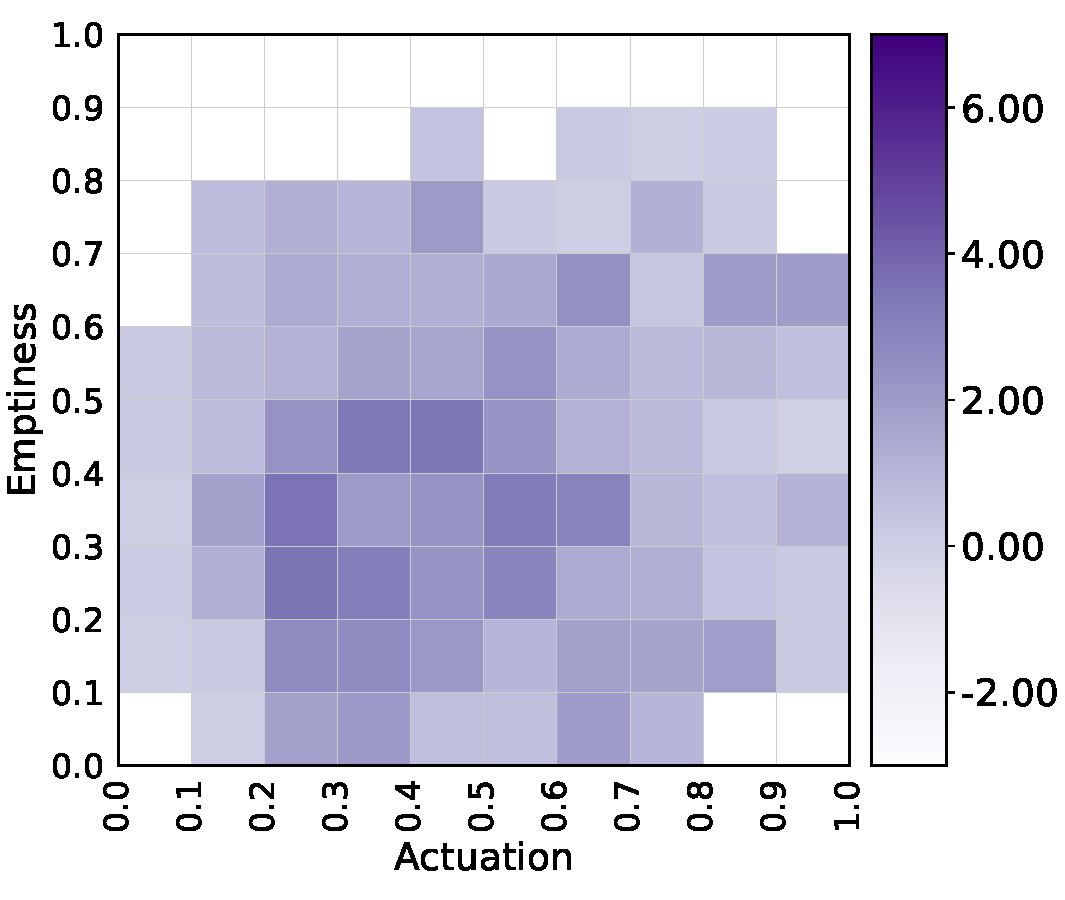
\includegraphics[scale=0.3]{images/multitasking/carrier_w.pdf}
         \caption{Walker}
         \label{carrier_a}
    \end{subfigure}
    \hfill
    \begin{subfigure}[b]{0.3\textwidth}
         \centering
         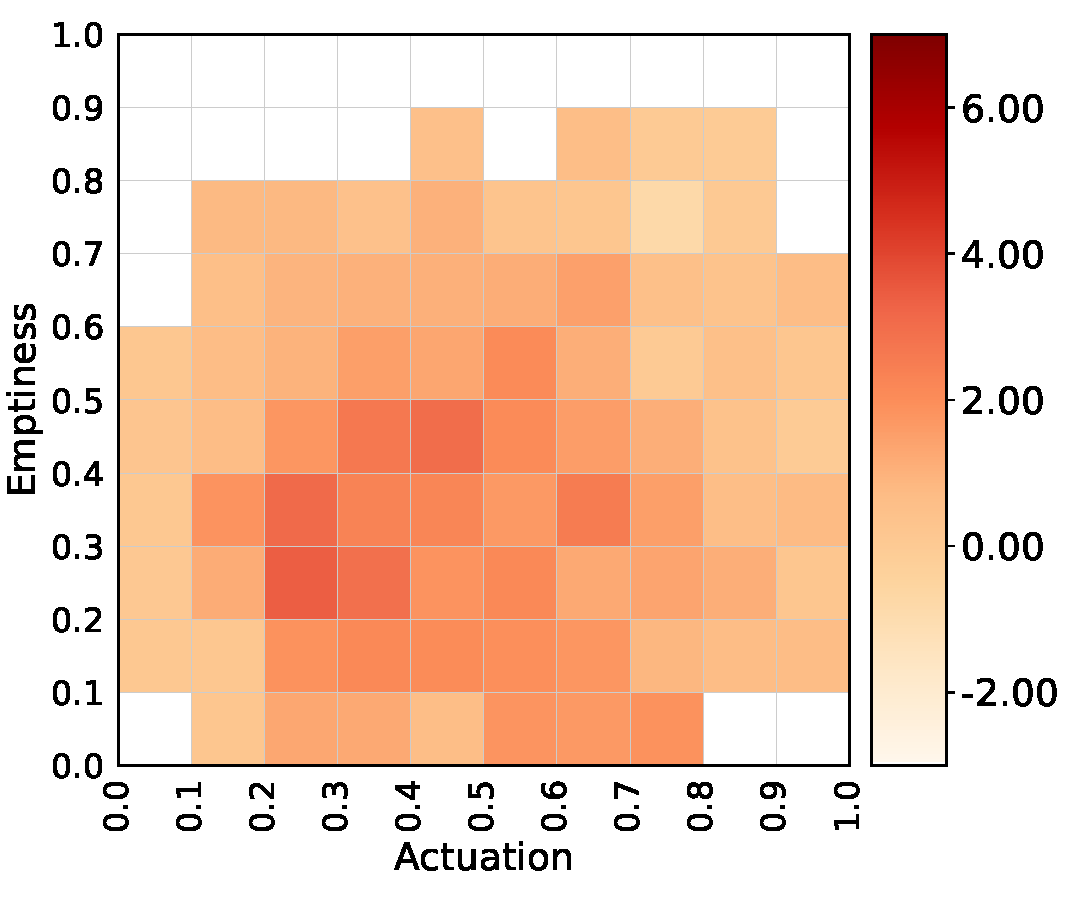
\includegraphics[scale=0.3]{images/multitasking/carrier_p.pdf}
         \caption{Pusher}
         \label{carrier_b}
    \end{subfigure}
    \hfill
    \begin{subfigure}[b]{0.3\textwidth}
         \centering
         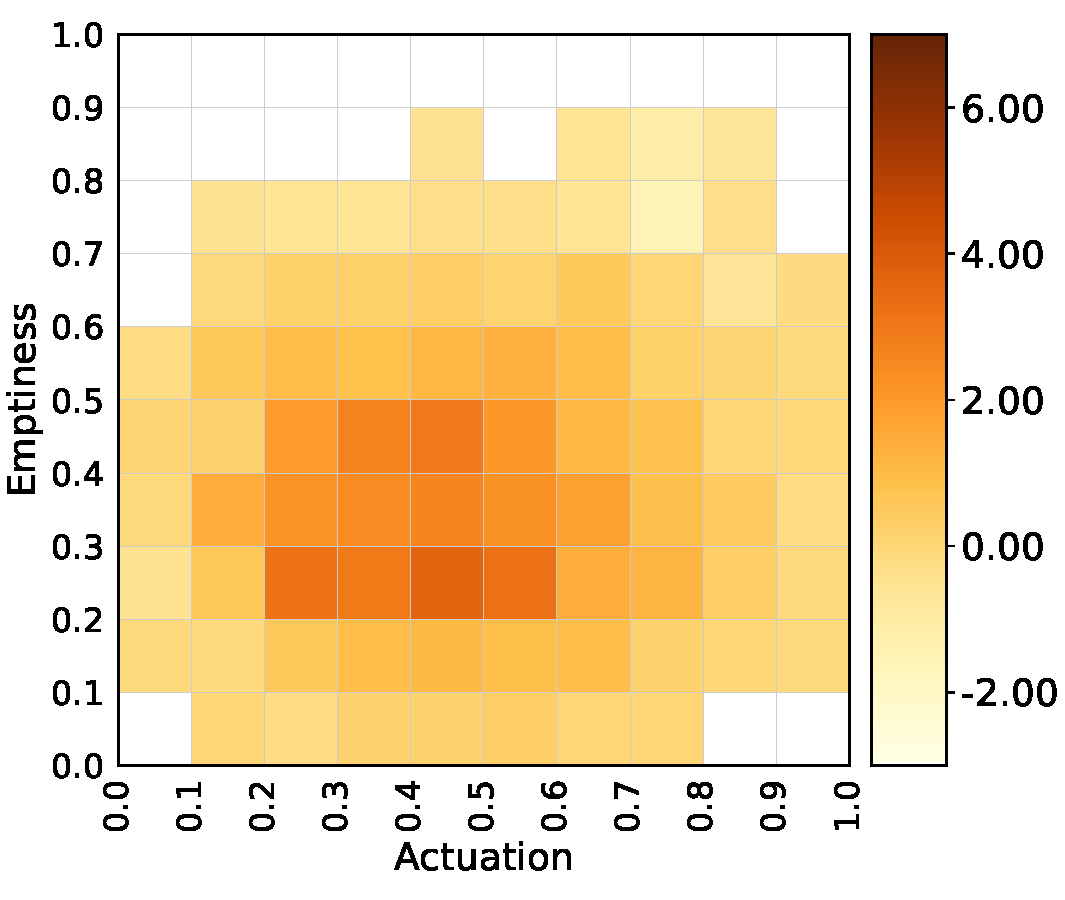
\includegraphics[scale=0.3]{images/multitasking/carrier.pdf}
         \caption{Carrier}
         \label{carrier_c}
    \end{subfigure}
    \caption{Carrier designs trained in the walker (a), pusher (b), carrier (c) task.
    The maps can be compared for the fitness distribution, however the obtained fitness cannot be compared, since its definition is different in the three tasks.}
    \label{fig:carrier_multitask}
\end{figure}


Table \ref{tab:results} provides the numerical results of these experiments.
Each row defines where the designs of the individuals have been optimized, the columns refer to the environment on which the individuals have been evaluated.

Each cell indicates the mean and the standard deviation of the designs best performing in the environment in row, trained in the task in column.
The value of each cell has been computed by considering all the individuals in the final map of six experiments, launched with different seeds. The respective mediated maps are the ones shown in Figures \ref{fig:walker_multitask}, \ref{fig:pusher_multitask}, \ref{fig:carrier_multitask}.

The table confirms that for each task the greatest rewards are obtained by the individuals for which the body and the controller have been optimized in that same environment.

Note the the results in row are not comparable, since each task has its own definition of reward, defined in Chapter \ref{cha:chapter1}.

\begin{table}[h]
    \centering
    \begin{tabular}{r|c|c|c|}
         & Walker task & Pusher task & Carrier task \\
         \hline
        Walker & $3.913 \pm 2.21$ & $ 1.7\pm1.391 $ & $-0.602 \pm 0.938$\\
        Pusher & $  2.297\pm1.989 $ & $2.713 \pm 1.533$ & $-0.424 \pm 0.975$ \\
        Carrier & $ 1.481\pm1.634 $ & $ 1.275\pm1.237 $ & $0.801 \pm 1.286$ \\
        \hline
    \end{tabular}
    \caption{Comparison of task performance.
    Each row defines where the bodies have been optimized; each column refers to the environment on which the controllers have been trained, and where the individuals have been evaluated.
    Each cell indicates the mean and standard deviation.
    Please note the the results in row are not comparable since each task defines its own reward.}
    \label{tab:results}
\end{table}



\section{Validating or training in a new task}
The carrier and pusher task have the same observation space, therefore it's possible to use both the body and the controller optimized in an environment on the other task.

%%% CARRIER %%%
The best performing carriers get a higher fitness value in the pusher task if their controller is trained in the new environment, as shown in Figure \ref{fig:carrier_val_tr}.\\
The first row in Table \ref{tab:carrier_pusher_results} confirms that the mean fitness is greater when the controller is optimized in the new environment, but it also shows that it has a greater standard deviation.

\begin{figure}[H]
    \centering
    \begin{subfigure}[b]{0.49\textwidth}
         \centering
         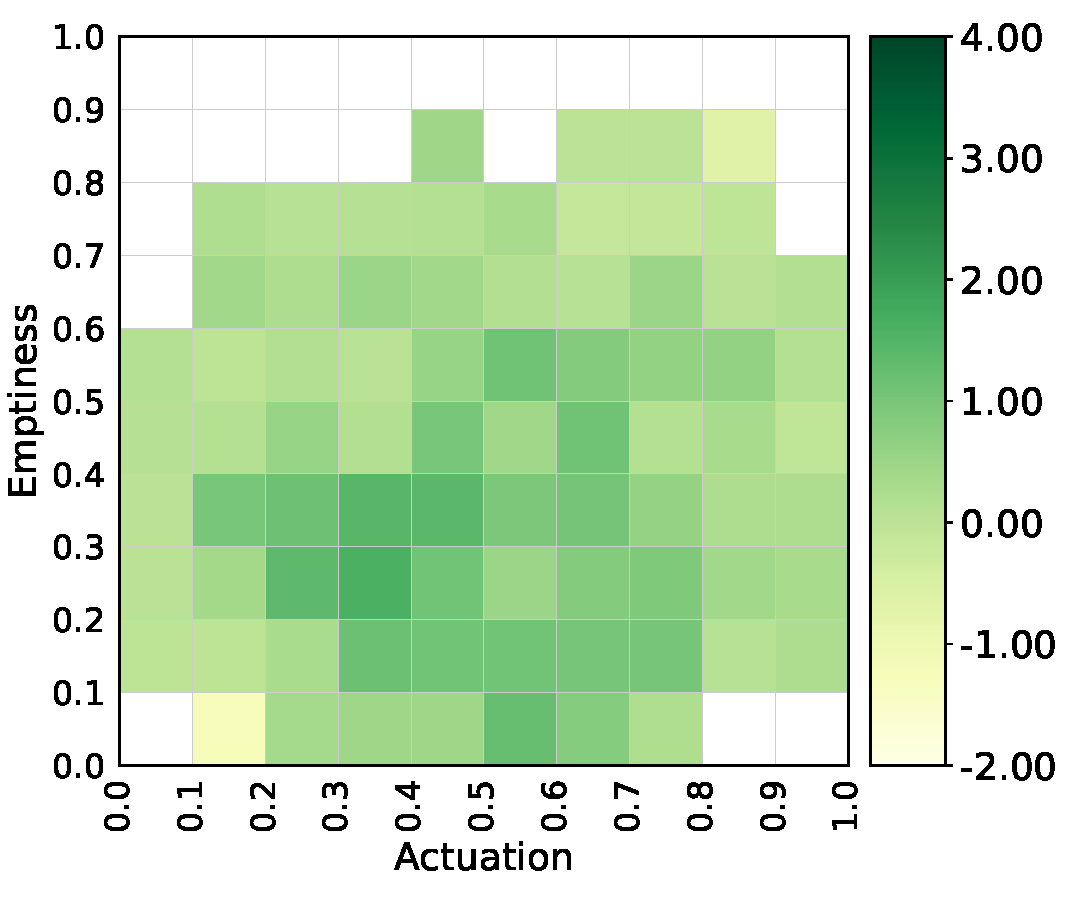
\includegraphics[scale=0.4]{images/multitasking/carrier_val_p.pdf}
         \caption{Validation}
    \end{subfigure}
    \hfill
    \begin{subfigure}[b]{0.49\textwidth}
         \centering
         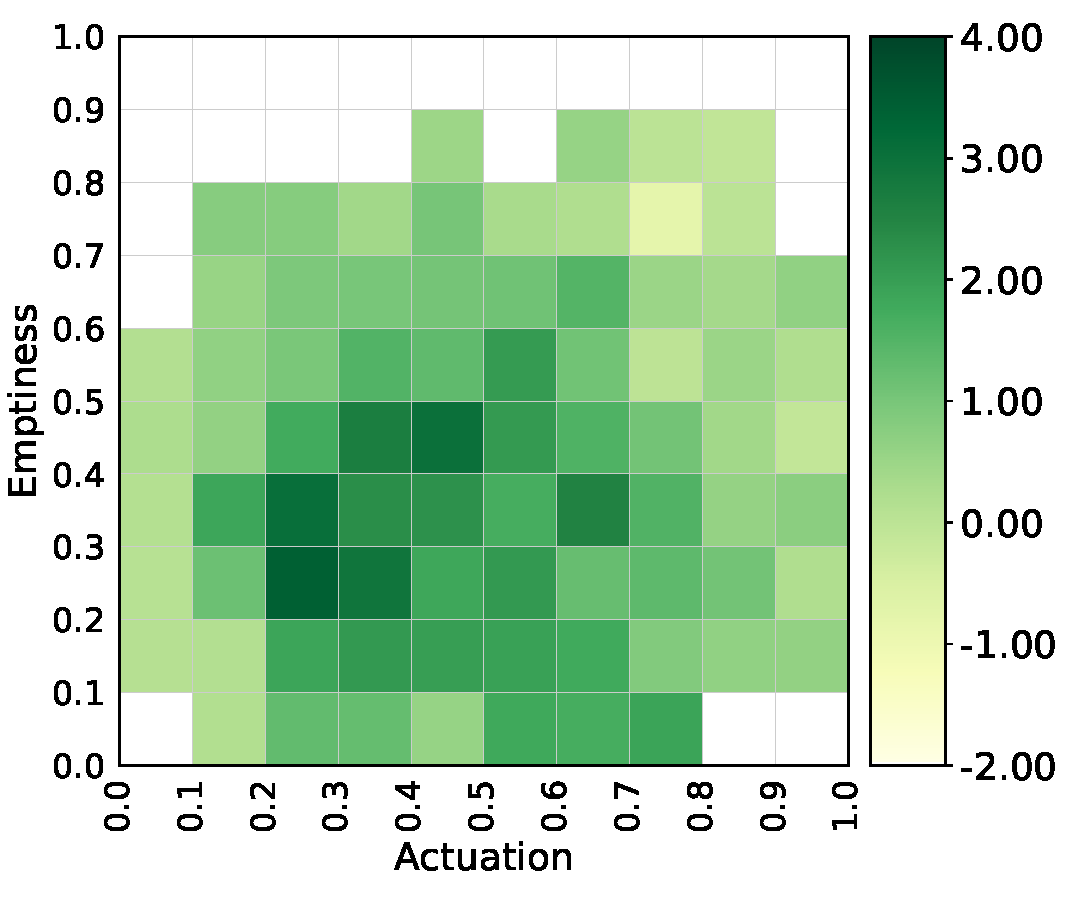
\includegraphics[scale=0.4]{images/multitasking/carrier_tr_p.pdf}
         \caption{Controller training}
    \end{subfigure}
    \caption{Performances of the best carrier designs in the pusher task.  The the performances of individuals are improved when controllers are trained in the new task (b), compared with the validation only (a).}
    \label{fig:carrier_val_tr}
 \end{figure}

\begin{figure}[h]
    \centering
    \begin{subfigure}[b]{0.49\textwidth}
         \centering
         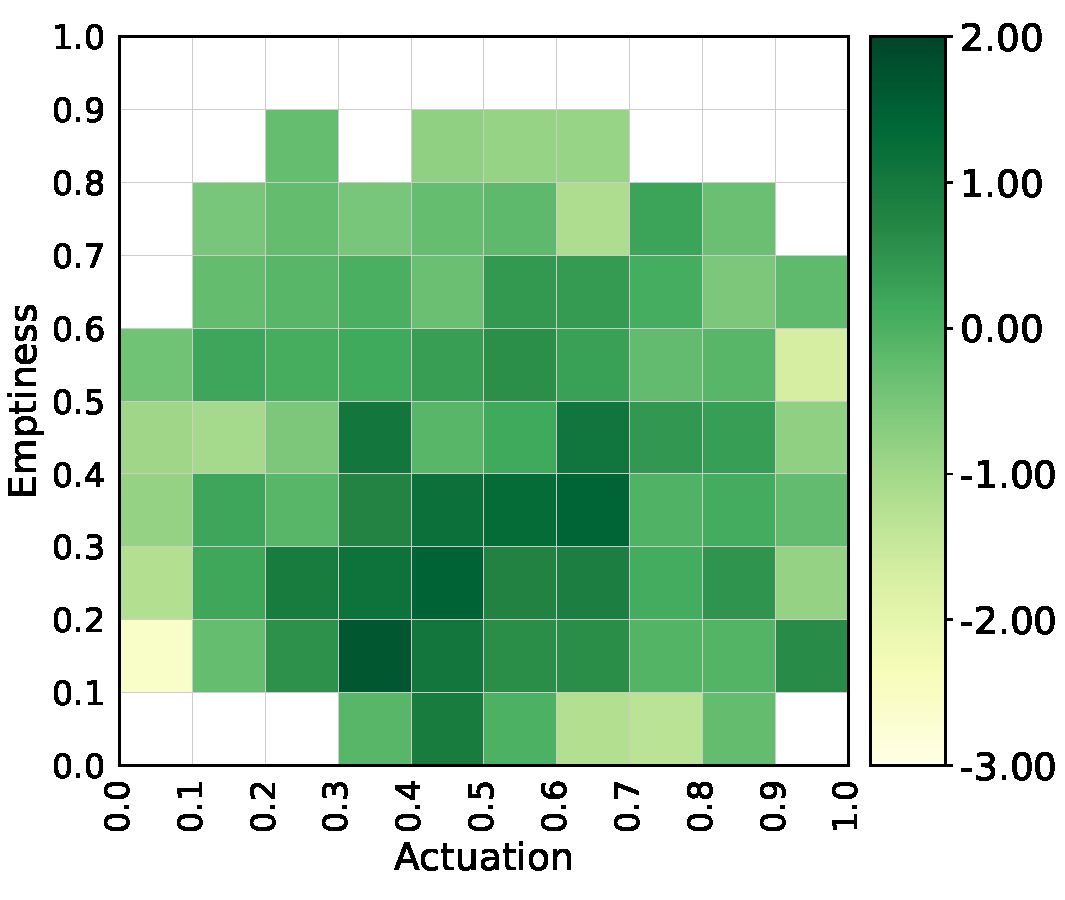
\includegraphics[scale=0.4]{images/multitasking/pusher_val_c.pdf}
         \caption{Validation}
    \end{subfigure}
    \hfill
    \begin{subfigure}[b]{0.49\textwidth}
         \centering
         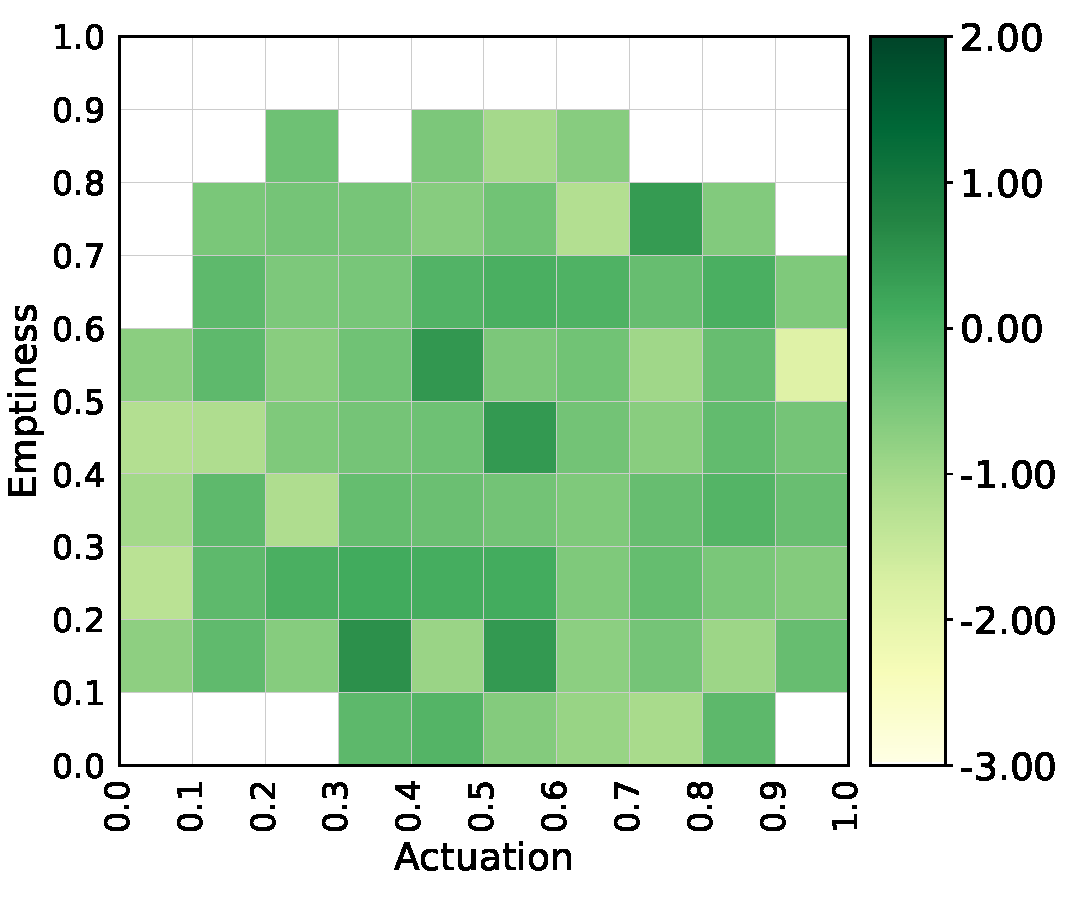
\includegraphics[scale=0.4]{images/multitasking/pusher_tr_c.pdf}
         \caption{Controller training}
    \end{subfigure}
    \caption{Performances of the best pusher designs in the carrier task. The comparison shows that simply validating individuals (a) gets better results than training controllers (b) in the new task.}
    \label{fig:pusher_val_tr}
 \end{figure}
 
%%% PUSHER %%%
Figure \ref{fig:pusher_val_tr} provides a comparison of the best pusher designs validating and optimizing the controller in the carrier task.\\
Contrary to the considerations for the carrier designs in the pusher task, the two maps highlight that the validated individuals perform better than the ones whose controller has been trained in the new task.\\
The results are confirmed by computing the mean of the fitness, as shown in the second row in Table \ref{tab:carrier_pusher_results}. However, the table also points out that not optimizing the controller leads to a greater standard deviation.\\
The greater result with no further optimization is due to the pushers walking ability: since a component of the carrier task reward consists of the position of the robot, this ability allows it to get a good fitness value, despite the behaviour of the box.
 
\begin{table}[H]
    \centering
    \begin{tabular}{|l|c|c|}
    \cline{2-3}
    \multicolumn{1}{c|}{} & \multicolumn{1}{c|}{validation} & \multicolumn{1}{c|}{optimization}\\
    \hline
        carrier designs & $ 0.54 \pm 0.84 $ & $ 1.275 \pm 1.237 $ \\
        \hline
        pusher designs & $ 0.124 \pm 1.369 $ & $ -0.424 \pm 0.975 $ \\
    \hline
    \end{tabular}
    \caption{Carrier and pusher multitask experiments.
    Mean and standard deviation for the experiments with validation only or with the controller optimization in the new task.
    The first row shows the results of the best carrier designs in the pusher task, the second row refers to the best pusher designs in the carrier task.}
    \label{tab:carrier_pusher_results}
\end{table}


\section{Conclusion}
This chapter introduced some considerations about using the same designs in various tasks.

The best results in each environment are obtained when the body and the controller are both optimized in the same task, confirming that the robot co-optimization is strongly connected to the environment definition.

The pusher and carrier tasks showed that it's also possible to perform well on a new task even with no controller re-optimization; however, since it doesn't provide excellent results, further analysis might provide interesting and surely more precise information.

The reward definition of the task on which individuals are evaluated greatly affects the results.
About this, it was shown that the best pusher designs can get a great reward in the carrier task even with no controller optimization in the new environment, due to their ability to walk, which increases the final reward value in spite of the penalty applied for dropping the box.

\newpage